% SPDX-License-Identifier: CC-BY-SA-4.0
% Session: Form parallelism to concurrency
% Exercise: Amdahl's law

\begingroup

\begin{exercice}[Skip list] Présentation selon Wikipédia :
  \og Une skip list se présente comme une amélioration d'une liste chaînée triée.
  Elle contient des pointeurs supplémentaires vers l'avant, ajoutés de façon aléatoire,
  de sorte que la recherche dans la liste puisse ``sauter'' (to skip en anglais) de nombreux éléments.

  La skip list est organisée en couches. La couche la plus basse est simplement une liste chaînée standard.
  Chaque couche supérieure $i+1$ est une ``voie rapide'' pour parcourir les couches inférieures $0, \dots, i$.
  Un élément présent sur la couche $i$ a une probabilité fixée $p$ de faire partie de la couche $i+1$.
  En moyenne, chaque élément apparaît dans $\frac{1}{1-p}$ listes, et l'élément le plus haut
  (souvent un élément factice plus petit que tous les autres) apparaît dans $\mathcal{O}\left(\log_{\frac{1}{p}}(n)\right)$ couches.
  \fg

  La figure ci-dessous représente l'une des structures possibles encodant l'ensemble $\{0,10,25,30,50\}$.
  
  \vspace{2mm}

  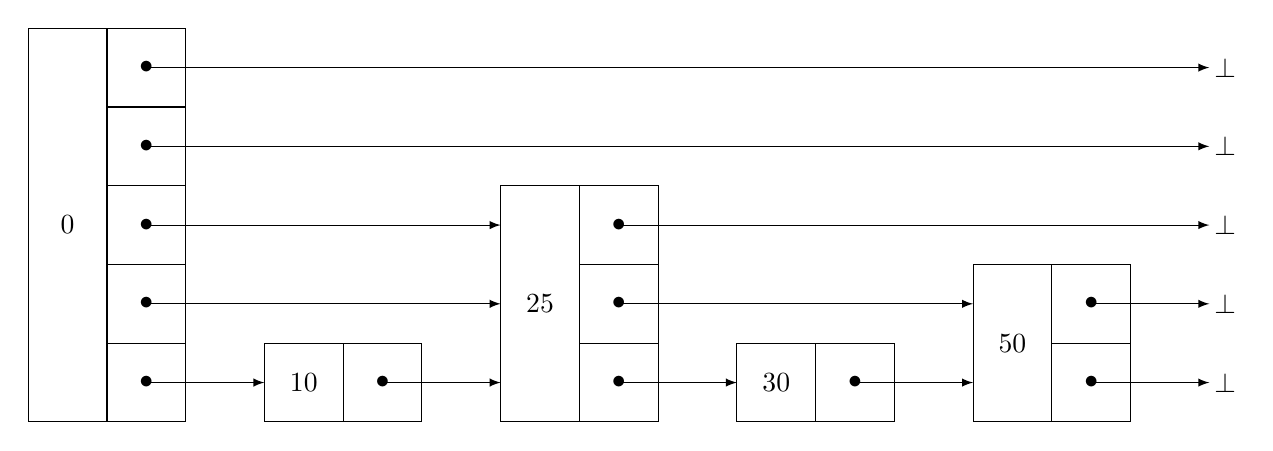
\begin{tikzpicture}
    \draw (0,0) rectangle (2,5);
    \draw (1,0) -- (1,5);
    \draw (1,1) -- (2,1);
    \draw (1,2) -- (2,2);
    \draw (1,3) -- (2,3);
    \draw (1,4) -- (2,4);
    \draw (0.5,2.5) node{0};
    \draw[-latex] (1.5,4.5) node{$\bullet$} -- (15,4.5);
    \draw[-latex] (1.5,3.5) node{$\bullet$} -- (15,3.5);
    \draw[-latex] (1.5,2.5) node{$\bullet$} -- (6,2.5);
    \draw[-latex] (1.5,1.5) node{$\bullet$} -- (6,1.5);
    \draw[-latex] (1.5,0.5) node{$\bullet$} -- (3,0.5);

    \draw (3,0) rectangle (5,1);
    \draw (4,0) -- (4,1);
    \draw (3.5,0.5) node{10};
    \draw[-latex] (4.5,0.5) node{$\bullet$} -- (6,0.5);

    \draw (6,0) rectangle (8,3);
    \draw (7,0) -- (7,3);
    \draw (7,1) -- (8,1);
    \draw (7,2) -- (8,2);
    \draw (6.5,1.5) node{25};
    \draw[-latex] (7.5,2.5) node{$\bullet$} -- (15,2.5);
    \draw[-latex] (7.5,1.5) node{$\bullet$} -- (12,1.5);
    \draw[-latex] (7.5,0.5) node{$\bullet$} -- (9,0.5);

    \draw (9,0) rectangle (11,1);
    \draw (10,0) -- (10,1);
    \draw (9.5,0.5) node{30};
    \draw[-latex] (10.5,0.5) node{$\bullet$} -- (12,0.5);

    \draw (12,0) rectangle (14,2);
    \draw (13,0) -- (13,2);
    \draw (13,1) -- (14,1);
    \draw (12.5,1) node{50};
    \draw[-latex] (13.5,1.5) node{$\bullet$} -- (15,1.5);
    \draw[-latex] (13.5,0.5) node{$\bullet$} -- (15,0.5);

    \draw (15.2,4.5) node{$\bot$};
    \draw (15.2,3.5) node{$\bot$};
    \draw (15.2,2.5) node{$\bot$};
    \draw (15.2,1.5) node{$\bot$};
    \draw (15.2,0.5) node{$\bot$};
  \end{tikzpicture}

  \begin{question}
  \item Proposez une implémentation linéarisable et lock-free de la skip list. On prendra $p=\frac{1}{2}$, et on pourra fixer la taille de la couche la plus haute à $32$. 
  \end{question}

\end{exercice}

\endgroup
\endinput
